% options:
% thesis=B bachelor's thesis
% thesis=M master's thesis
% czech thesis in Czech language
% slovak thesis in Slovak language
% english thesis in English language
% hidelinks remove colour boxes around hyperlinks

\documentclass[thesis=M,czech]{FITthesis}[2012/06/26]

\usepackage[utf8]{inputenc} % LaTeX source encoded as UTF-8

\usepackage{graphicx} %graphics files inclusion
% \usepackage{amsmath} %advanced maths
% \usepackage{amssymb} %additional math symbols

\usepackage{dirtree} %directory tree visualisation

% % list of acronyms
% \usepackage[acronym,nonumberlist,toc,numberedsection=autolabel]{glossaries}
% \iflanguage{czech}{\renewcommand*{\acronymname}{Seznam pou{\v z}it{\' y}ch zkratek}}{}
% \makeglossaries

\newcommand{\tg}{\mathop{\mathrm{tg}}} %cesky tangens
\newcommand{\cotg}{\mathop{\mathrm{cotg}}} %cesky cotangens

% % % % % % % % % % % % % % % % % % % % % % % % % % % % % % 
% ODTUD DAL VSE ZMENTE
% % % % % % % % % % % % % % % % % % % % % % % % % % % % % % 

\department{Katedra \ldots (Softwarového inženýrství)}
\title{Distrubuované ukládání a zpracování velkého množství dat - případové studie}
\authorGN{Dominik} %(křestní) jméno (jména) autora
\authorFN{Veselý} %příjmení autora
\authorWithDegrees{Bc. Dominik Veselý} %jméno autora včetně současných akademických titulů
\supervisor{Ing. Michal Valenta, PhD}
\acknowledgements{Doplňte, máte-li komu a za co děkovat. V~opačném případě úplně odstraňte tento příkaz.}
\abstractCS{V~několika větách shrňte obsah a přínos této práce v~češtině. Po přečtení abstraktu by se čtenář měl mít čtenář dost informací pro rozhodnutí, zda chce Vaši práci číst.}
\abstractEN{Sem doplňte ekvivalent abstraktu Vaší práce v~angličtině.}
\placeForDeclarationOfAuthenticity{V~Praze}
\declarationOfAuthenticityOption{4} %volba Prohlášení (číslo 1-6)
\keywordsCS{Nahraďte seznamem klíčových slov v češtině oddělených čárkou.}
\keywordsEN{Nahraďte seznamem klíčových slov v angličtině oddělených čárkou.}

\begin{document}
	
% \newacronym{CVUT}{{\v C}VUT}{{\v C}esk{\' e} vysok{\' e} u{\v c}en{\' i} technick{\' e} v Praze}
% \newacronym{FIT}{FIT}{Fakulta informa{\v c}n{\' i}ch technologi{\' i}}

\begin{introduction}
	%sem napište úvod Vaší práce
\end{introduction}



\chapter{Cíl práce}
Zmínit že práce nikterak nesrovnává klasické a BigData databáze naopak se zabývá open source nástroji od apache


\section{Motivace}
\section{Příprava předmětu}
\section{Rozšíření povědomí}
\section{Praktické zkušenosti}


\chapter{Co jsou to BigData}



Popsat termín BigData není úplně snadné, a to hned z~několika důvodů. Především proto, že neexistuje žádná přesná definice tohoto pojmu. Tento termín je stejně jako obor, kterého se týká, velice dynamický a rychle se mění. K~obtížnější definici pojmu přispívá také fakt, že se hojně používá v~marketingové komunikaci jako tzv. \uv{buzzword} za účelem vzbudit zájem čtenáře/posluchače, přestože může být použit v~nesprávném kontextu.

Termín BigData označuje manipulaci s~datasety tak velkými, že je nemožné nebo velice obtížné s~nimi manipulovat za pomocí tradičních nástrojů a databází (převážně relačních). Pod pojmem manipulace s~datasety myslíme:

\begin{itemize}
  \item Sběr
  \item Organizace
  \item Ukládání
 \item Prohledávání
 \item Sdílení
 \item Analýza
 \item Vizualizace
\end{itemize}

Nalezení této hranice či její přesná definice je komplikovanější problém mimo rozsah této práce. Na toto téma již bylo publikováno mnoho jiných prací. Jak jsem zmínil již v~úvodu, práce se dále také nezabývá porovnáním BigData a klasických relačních databází. 

V~této kapitole se pokusím obecně přiblížit, co to tedy BigData jsou, jak se liší a důvod vzniku tohoto odvětví.


\section{Trend velkých datasetů}
Jak jsem již naznačil, BigData se věnují zpracování velkých datasetů. Trend upřednostňování velkých datasetů oproti několika menším, které v~součtu mají stejný objem a nesou stejné množství informace, začal vzhledem k~jednoduššímu hledání a objevení i zdánlivě neexistujících korelací, projevení obchodních trendů a vyhodnocování dat v~reálném nebo skoro reálném čase.

\section{3V}
Jak naznačil předchozí odstavec, BigData nejsou pouze o~objemu zpracovávaných dat, jak by se na první pohled mohlo zdát. Jedná se o~komplexnější kategorizaci, kde hrají roli i ostatní charakteristiky, které se v~literatuře značí zkratkou 3V, odvozenou od počátečních písmen těchto kategorií v~anglickém jazyce.

\begin{figure}[h]
\centering
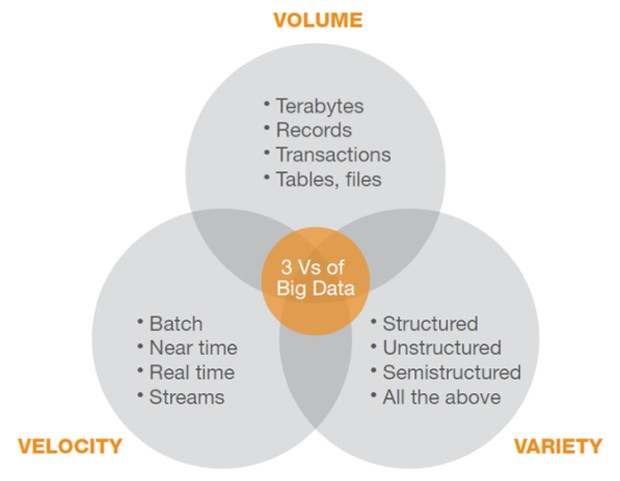
\includegraphics[scale=0.6]{images/3v}
\caption{Schéma popisující 3V pomocí množinových diagramů \cite{3vimg}}
\label{fig:3v}

\end{figure}

\subsection[3v-volume]{Obsah (Volume)}
Data se dnes zdaleka nevyskytují jen v~textové podobě, můžeme je uchovávat formou hudby, obrázku či videa. Vzhledem k~tomuto faktu čelíme exponenciálnímu nárůstu množství uchovávaných dat a není výjimečné, aby enterprise systémy uchovávaly terabyty nebo petabyty dat. Data tedy tvoří množství informací, které je dost často vyhodnocováno z~různých úhlů a následně uloženo a znovu vyhodnocováno, a přestože původní data zůstala nezměněna, díky reevaluaci nám jejich množství roste závratným způsobem. Tímto způsobem může být na objem nahlíženo jako na jednu z~charakteristik BigData.

\subsection{Rychlost (Velocity)}
Na rychlost můžeme nahlížet hned ze dvou pohledů. Prvním pohled vyjadřuje rychlost, jakou nám data přibývají a jak aktuální pro nás jsou. Například historie vývoje měnového kurzu je informace, jejíž včerejší hodnota je naprosto nevypovídající a mění se s~každou minutou. Změnila se i rychlost, jakou noviny a televizní stanice získávají informace skrze sociální sítě. Objem dat tedy roste rychle a aktuálnost informací se rapidně zkrátila. Druhý pohled na tuto charakteristiku se zabývá rychlostí, jakou data potřebujeme zpracovávat. Jsou informace, které k~nám proudí velice často (například každou minutu), ale jejich vyhodnocení dává smysl ku příkladu jen jednou za 24 hodin. Ovšem jsou také data, které potřebujeme zpracovávat v~reálném čase, tak, jak k~nám proudí. Dobrým příkladem takových dat mohou být akutální informace z~meteorologické stanice. 
Rychlost, v~jaké jsou dnes data zpracovávána, se mnohonásobně zmenšila a tedy nejen objem dat, ale i rychlost zpracování reprezentuje samotná BigData.

\subsection{Různorodost (Variety)}
Jak je z~Obrázku ~\ref{fig:3v} patrné, různorodost dat znamená jejich strukturovanost/nestrukturovanost. Již bylo zmíněno, že data mohou mít mnoho podob. Ale i data ve stejné podobě (například textové), mohou být jinak strukturována a tomuto faktu je potřeba se přizpůsobit a uchovávat a zpracovávat data v~jiných formátech.
Různorodost a adaptabilita jsou tedy posledními charakteristikami BigData.

\section{BigData zjednodušeně}
Předcházející řádky by měly sloužit jako shrnutí a lehký úvod do problematiky BigData. Dalo by se vlastně také říci, že BigData nejsou jen o~velkém množství dat, ale je to celý koncept uchovávání a možností nových náhledů na stávající data, ale také návod, jak zachytit a zpracovat budoucí data. Další odstavce budou věnovány historii tohoto konceptu, ale také nejtypičtějších odvětví, kde se s~ním můžeme setkat. 

\section{Historie}

Již od počátků počítačové éry bylo potřeba data analyzovat. \cite{history} S~rychle se zvyšující dostupností moderních technologií a jejich obecnému přijetí ve společnosti, se posouvaly hranice této potřeby od vládních organizací až po současnost, kdy obrovské množství informací a jejích analýzu potřebují i malé podniky.

\subsection{30. a 40. léta}
V~této době se používaly první počítačové simulace. Prim hrálo především válečné odvětví, kde například vědci z~projektu Manhattan pomocí počítačových simulací simulovali dopad a následný zničující efekt jaderné bomby.

\subsection{50. a 60. léta}
V~tomto období se počítače (a s~nimi také zpracování a analýza dat) rozšířily do velkých korporací a výzkumných laboratoří. Počítač ENIAC například generoval první modely pro předpověď počasí. Analytici také vyřešili první problém nejkratší cesty a mnoho dalších, viz. také \cite{history}.

\subsection{70. až 90. léta}
V~této době se analytická činnost rozšířila o~středně velké podniky a technologické startupy. Objevují se také dnes již dobře známé případy užití. Dobrým příkladem takových případů je třeba první predikční model na pokles a růst akcií. Dále také stojí za zmínku první komerční nástroj pro modelově řízené rozhodování. Důležitým milníkem je rovněž vznik společností, jako je Ebay a Amazon. Bitva o~personalizaci online nákupů právě začala! Google implementuje první vyhledávací algoritmus, který zvyšuje relevanci výsledků.

\subsection{2000 až součanost}
V~tomto období se analytika rozšířila až na oblast malých podniku a analytických expertů (jednotlivců). Začíná mít obrovský dopad na život každého z~nás. Samozřejmostí začínají být dynamické změny cen zboží, doporučování produktů, hudby a filmů nebo řízení dopravy. Rozvíjejí se obory, jako je analýza a procesování přirozeného jazyka z~novin, e-mailů nebo sociálních sítí. Příchodu BigData, vzhledem k~levné dostupnosti výpočetního výkonu a rychlosti zpracování dat, již nic nestojí v~cestě.

\subsection{Budoucnost}
Předpokládá se, že v~budoucnu bude analytická činnost řídit každodenní rozhodování i na úrovni jednotlivců. V~běžném životě se přínos analýzy dat projeví například: Predikce v~policejní sféře a boji proti zločinu, výzkum ve zdravotnictví nebo kompletně personalizovaná zákaznická interakce i pro malé podniky a řetězce.

\section{Nástup sociálních sítí}
BigData zažila obrovský nástup také díky příchodu a masivnímu rozšíření sociálních sítí, a to hned ze dvou důvodů. Prvním důvodem je, že nástup sociálních sítí přilákal tisíce výzkumníků, kteří začali sbírat data z~Facebooku a Twitteru. Tito výzkumníci následně hledali různá spojení mezi zprávami a účty, z~kterých poté vyvozovali závěry ohledně těchto sociálních sítí. Další možností, k~čemu vytěžená data používali, bylo vytváření tzv. sociálních grafů. Historicky sbírali antropologové a sociologové data o~lidských vztazích skrze dotazníky, rozhovory, pozorování a experimenty. Dolováním dat ze sociálních sítí, kde lidé sdílejí mnoho detailů ze svých životů, se jim otevřel nový kanál, kde mají všechny tyto informace jednoduše k~dostání a stačí je pouze analyzovat.

V oblasti sociálních sítí existují 2 konkrétní druhy, které jsou z hlediska konceptu BigData zajímavé: \uv{Artikulované sítě} a \uv{Behaviorální sítě}. První kategorie znázorňuje sítě, kde uživatelé zadávají svá přátelství a konexe skrze technické mechanismy jako například: telefonní seznamy, emaily, seznamy přátel z~jiných sití atd. Druhou kategorií jsou sítě odvozené od komunikačních vzorců. Do této skupiny spadají uživatelé, kteří si píšou zprávy nebo jsou označení na společných fotkách. Obě tyto skupiny mají pro výzkumníky velký význam, přestože jím nepřikládají takovou váhu jako reálným osobním vztahům. \cite{social} 

Druhým důležitým aspektem, proč jsou sociální sítě pro BigData důležité, je fakt, že tyto sítě samy potřebují někde svá data uchovávat a zpracovávat. Technologické týmy stojící za těmito službami se tak ve značné míře podílejí jako kolaborátoři na BigData projektech či dokonce vytvářejí a následně uvolňují svoje technologie k~užití pro širokou veřejnost. Pro komunitu jsou důležité i přednášky a prezentované poznatky od těchto datových gigantů, kteří prozkoumávají a prolamují lidstvu dosud známe bariéry a umožňují tím využívání technologických pokroků i jiným subjektům. 

Sociální sítě samozřejmě nejsou jediným průkopníkem na poli BigData. Internetoví giganti jako Google, Amazon a Yahoo přispívají neméně výrazným dílem. Na sociálních sítích je však zajímavé to, že jejich data jdou do jisté míry jednoduše dolovat, díky čemuž vzniklo mnoho spolčeností, které se začaly jejich analýzou a sběrem zabývat a způsobily tím popularizaci spojení BigData se sociálními sítěmi. 


\section{Odvětví}

Jak již bylo zmíněno v~předchozí sekci, v~dnešní době můžeme na BigData narazit kdekoliv. Zde bych chtěl poukázat na široké spektrum využití napříč různými činnostmi, kterými se lidstvo zaobírá.\cite{sektory}

\subsection{Maloobchod}
Péče o~zákazníka a samozřejmě také zvýšení zisku jsou hlavními motivy pro zpracovávání a analýzu dat. Na základě chování uživatelů (aktivita na webu, zákaznická karta, anonymní zákazníci) můžeme předpovídat chování zákazníka v~každém stádiu nákupu. Toto chování lze navázat také na podniková data a hledat korelace pomocí Map Reduce mechanismů. Největším průkopníkem spojování BigData a maloobchodu je bezesporu řetězec Tesco se svou věrnostní kartou ClubCard. Na základě zákazníkovy nákupní historie sestavují žebříček produktů k~doporučení či dokonce dokáží odhadnout období těhotenství svých zákaznic.\cite{tesco}

\subsection{Věda a výzkum}

Není žádným překvapením, že ve vědě a výzkumu se využívají BigData na uchovávání výsledků z~měření či pro hledání korelací v~naměřených hodnotách. Držitel Nobelovy ceny Peter Higgs používal NoSQL databázový systém Cassandra na zpracování svých dat, díky nímž prokázal existenci tzv. Higgsova Bosonu \cite{higgs}.

\subsection{Meteorologie}
Díky sběru a vyhodnocování dat z~meteorologických stanic se podařilo vytvořit mnohem spolehlivější a přesnější modely pro předpovědi počasí, a to jak dlouhodobých, tak také krátkodobých. 

\subsection{Finance}
Ve finančním sektoru je způsobů využití hned několik. Například již výše zmíněné doporučování produktů dle historie transakcí a sběru  osobních dat. Banky a jiné finanční instituce podobným způsobem nabízejí zákazníkům vhodné finanční produkty, jako jsou například hypotéky. Mnohem zajímavějším případem využití BigData je detekce podvodů, kdy jsou banky na základě analýzy všech transakcí schopny hledat vzory podvodných chování a vyhodnotit určité transakce jako podezřelé a tím tak chránit své klienty nebo samy sebe.

\subsection{Webová optimalizace}
Na základě ukládání a následného zpracování veškerého chování uživatele na stránce mohou firmy optimalizovat webové stránky a jejich obsah či ho případně restrukturalizovat. Po vyhodnocení chování konkrétních uživatelů je možné jim obsah stránky automaticky personifikovat a podsouvat tak uživatelům pro ně zajímavé věci, aniž by se k~nim museli složitě proklikávat.

\subsection{BioInformatika}
V~bioinformatice se BigData využívají například k~mapování genomů nebo k~sekvenční analýze. Tyto informace pomáhají k~lepšímu pochopení DNA a také k~prevenci genetických poruch a vrozených nemocí či k~usnadnění jejich léčby. \cite{industries} 

\section{Dnešní možnosti}
V~dnešní době existují v~podstatě 3 možnosti jak začít s~BigData. 

\subsection{Specializované firmy a hotová řešení}
Na internetu nalezneme několik firem zabývajících se analýzou vašich dat, kde veškerá analýza a vizualizace probíhá v~softwaru třetí strany. Mezi nejznámější patří společnost Good Data \cite{gooddata}. Tyto firmy se však specializují na zpracování firemních dat a vizualizaci v~jejich vlastních BI nástrojích.

\subsection{Hotová enterprise řešení}
Další možností je vybrat nějaké komplexní řešení od firem zabývajících se platformou BigData, které vám dodají software pro ukládání, analýzu a vizualizaci vašich dat. Programování komponent či jejich konfigurace je v~režii zákazníka a tyto firmy poskytují licence, školení a technickou podporu. Tuto možnost poskytuje například IBM.

\subsection{Open Source a řešení z~něj vycházející} 
Poslední možností je použití Open Source nástrojů, které umožní ukládat, analyzovat a vizualizovat data. Toto je cesta, kterou jsem se vydal v~rámci této práce a budu se jí tak nadále věnovat. Drobnou nadstavbou těchto řešení mohou být firmy nabízející komerční balíčky těchto Open Source řešení. Jedná se o~velice populární přístup v~případech, kdy je potřeba zkombinovat několik nástrojů dohromady. Jejich konfigurace bývá velice obtížná, a proto tyto komerční balíčky nabízí již nakonfigurovaná hotová řešení většinou i s~drobnou nadstavbou, která umožňuje provádět některé nadstandardní procesy a činnosti. 



%mozna jen podsekce bigdata%
\chapter{BigData techniky}



Abychom mohli hovořit o konkrétních technologicích, musíme nejdříve definovat základní stavební technologické kameny, o které se BigData opírají. Jedná se o technologie a paradigmata vyvinutá technologickými giganty, kteří jako první naráželi na technologické hranice a posouvali je dál a tak se postupně rodily tyto technologie a paradigmata. Jejich pořadí se odvýjí od logické posloupnosti tak, jak spolu souvisí a navazují na sebe.    

\section{Distribuované systémy}
Distribuované systémy, jsou tématem, které zasahuje samozřejmě mnohem dále, než jen do kategorie big data. Pro zjednodušení následujících řádků, zavedeme následující rozdělení. Distribuované systémy rozdělíme na systémy s distribuovaným výpočetním výkonem, systémy s distribuovaným úložištěm a nebo kombinace obojího. 

Distribuovaný výpočetní výkon, je takový systém, kde se výpočet jedné úlohy rozloží na více počítačů. Paralelní výpočety jsou známé z oblasti informačních technologií, již mnoho let a používají se nejčastěji k vědeckým výpočtům, paralelní kompilaci zdrojových kódů a nebo k jiným operacím, které by na jednom počítači trvaly příliš dlouho. 

Distribuované úložistě je jednoduše představitelné a důvodů mít data na více místěch je hned několik.
\begin{itemize}
\item Záloha - i ze sféry osobních počítačů známé trend kde máme data zálohovaná na více fyzických zařízeních, abychom předešli jejich ztrátě, v případě technické poruchy na daném zařízení. 

\item Nedostatek kapacity - Ze sféry osobních počítačů známe, že uživatelé, méně potřebné soubory ukládají na externí periferie, protože kapacita disků v osobních počítačích je zpravidla kolem pár TB.

\item Dostupnost - Pokud chce uživatel mít přístup k jednomu souboru z domácího i pracovního počítače, musí soubor mít fyzicky na těchto dvou počítačích, nebo využít nějaký software na sdílení souborů. 

\end{itemize}

Kombinovaný přístup je zřejmy a tedy, že se používá jak výpočetní výkon jednotlivých počítačů v systému, tak jejich úložný prostor. 

Big Data využívá všechny tyto přístupy, je zřejmé že obrovské množství dat, o kterém jsme mluvili v úvodu se lépe zpracovává na více počítačích. Stejně tak je logické, že pokud budeme bavit o množství dat, tak velké množství dat, uložíme na více počítačů, stejně tak pokud data chceme zálohovat. 

Ne vždy však využíváme kombinovaný přístup, je totiž velmi časté, že si firmy staví obrovské počítačové farmy, které slouží pouze jako datové sklady a datová centra. Vždy záleží na konkrétní situaci a způsobu využití. 


\section{CAP Theorem}
V roce 2000 při nástupu distribuovaných systémů vydal vědec Eric Brewer článek, popisucjíí tzv. CAP Theorem \cite{cap}, který se distribuovaných systémů přímo týká. Teorém říká, že distribuované systémy mají tyto 3 hlavní vlastnosti. 

\begin{itemize}
\item Konzistence (Consistency) - Vlastnost, která určuje, zda pro každý požadavek, vratí server správný výsledek. to znamena že odpověd je adekvátní vůči specifikaci požadované služby. Přesný význam konzistence se odvýjí od typu služby. V případě dat ji definujeme tak, že každý server má aktuální a stejná data.

\item Dostupnost (Availability) - Vlastnost která říka, že každý požadavek dostane odpověd. Rychlejší odpověd, je preferovanější oproti pomalejší, ale v kontextu teorému je důležité, že odpověd dorazí. V praxi však znamená, že velice opožděná odpověd je stejně spatná jako žádná odpověd a můžeme tuto vlastnost zjednodušit, že systém vždy musí být dostupný.

\item Tolerance výpadku (Partiotion tolerance) - Tato vlastnost jako jediná určuje chování podpůrného systému na kterém služba běží, namísto popisu chování služby samotné. Tato vlastnost říká, jestli během výpadku nějaké části systému, je systém schopný pokračovat a dále fungovat.

\end{itemize}


Brewer popisuje, že každý distribuovaný systém může splňovat nejvýše 2 z těchto 3 vlastností.

\subsection{CAP Theorem v roce 2012}
V roce 2012 napsal Brewer další článek \cite{cap2}, ve kterém popisuje stav jeho theorému po 12 letech. Vysvětluje, že již od začátku bylo označení \uv{pouze 2 ze 3} zavádějící a vágní, protože spoustu věcí příliš zjednodušovalo. Například u systému s velkou granularitou,  se mezi volbou C a A rozhoduje na několika úrovních a všechny vlastnosti mají spíše hodnoty v čase, než binární a také, že záleží na stavbě systému a jeho drobných nuancích. Také ale píše, že v důsledku theorém splnil svůj účel a otevřel tak systémévým návrhárům oči pri navrhování distribuovaných systémů a donutil je zamyslet se nad vyhodami a nevýhodami jednotlivých vlastnotí systému. 

V témže roce vyšel další zajímavý článek popisující aktuální stav CAP theorému \cite{cap3}. Popisuje převážně vztah
systémů k volbám CAP vlastnostní. 

\subsubsection{Nejlepší možná dostupnost}
Nejčastejší výběr je garantovaná konzistence s maximální možnou dostupností, pro většinu systémů je toto přirozenou volbou. Tedy, že za každou cenu, server vrací správnou odpověd a snaží se poté optimalizovat co největší dostupnost a nejrylechjší možnou odpověd vzhledem k síťovým podmínkám. Tento přístup dává největší smysl pokud jsou počítače ve stejném datacentru a běží na nich stejná služba. Typickým zástupcem je  \uv{lock service} a služba spravující metada pro nějaký distribuovaný systém s nízkou granularitou.

\subsubsection{Nejlepší možná konzistence} 
Druhou nejčastější skupinou jsou systémy, pro které je ztráta dostupnosti nemyslitelná a tudíž garantují dostupnost a snaží se o co nejvyšší úroveň konzistence. Tento postup nejlépe vyhovuje v případech kdy máme počítače distribuované napříč několika datacentry, v tomto případě může totiž dostupnost rapidně klesat s jakoukoliv chybou a proto je potřeba ji garantovat. V těchto případech tedy designéři obětují konzistenci, aby mohli garantovat dostatečně rychlou odpověd, přestože ta nemusí být vždy zcela správná. Ideálním příkladem jsou webové cache a obrázkové servery.

\subsubsection{Segmentovaná konzistence a dostupnost}
toto je nejzajímavější možnost a pro tuto práci je také nejdůležitější. Existují systémy, které nemají jednotné požadavky pro všechny aspekty služby. Některé vyžadují silnou konzistenci a některé vysokou dostupnost. Pro dodžení CAP theoremu se  jako nejpřirozenější možnost jeví rozdělit systém na několik jednotlivých komponent, které budou specificky nastaveny. tím tedy celý systém nezaručuje ani konzistenci, ani dostupnost, ale každá část systému postkytuje opravdu vlastnosti, které potřebuje. Segmentace může probíhat na několika možných úrovních. 

\begin{itemize}
\item \textbf{Rozdělení podle dat} - jiná data mohou vyžadovat jinou úroveň dostupnosti a konzistence.
\item \textbf{Rozdělení podle operací} - Operace pro zápis mohou mít jiné požadavky na konzistenci a dostupnost, než operace pro čtení.
\item \textbf{Rozdělení podle funkcí} - Některé služby mohou být rozděleny na podslužby a tedy pro každou takovouto službu můžeme mít vlastní úroveň konzistence a dostupnosti. 
\item \textbf{Rozdělení podle uživatelů} - Jedná se o rozdělení závislé převážně na geografické poloze uživatele, služba bude pro uživatele, který se nachází blízko může zaručit vysokou dostupnost a zároveň v rámci jeho blízkého data centra udržovat i konzistenci. 
\item \textbf{Rozdělení podle hierarchie} - Jedná se o systém ve kterém se na určitých úrovních kombinují výše popsané rozdělení.
 
\end{itemize}
\section{Distribuovaný file systém}

V předchozích sekcích jsme rozebrali distribuované systémy a jejich omezení. Zmínili jsme také, nutnost sdílet velké množství dat napříč několika počítači, které můžou být napříč různými datacentry. Tuto potřebu, tedy mít distribuovaný filesystém, měl i jeden z největších technologických gigantů, firma Google. V roce 2004, se Google rozhodl o jejich řešení podělit a vydal detailní článek \cite{gfs} popisující kompletní funkčnost a detaily celé infrasntruktury. Vysvětlení funkčnosti a  architektury je nad rámec této práce a navíc je vše dobře popsané v článku samotném, důelžité je však zmínit, že tento systém se stal inspirací a nastolil trend v tom, jak podobné systémy dnes vypadají a jaké mají vlastnosti. Na základě tohoto článku vznikl například opensource klon MooseFS.

\begin{figure}[h]
\centering
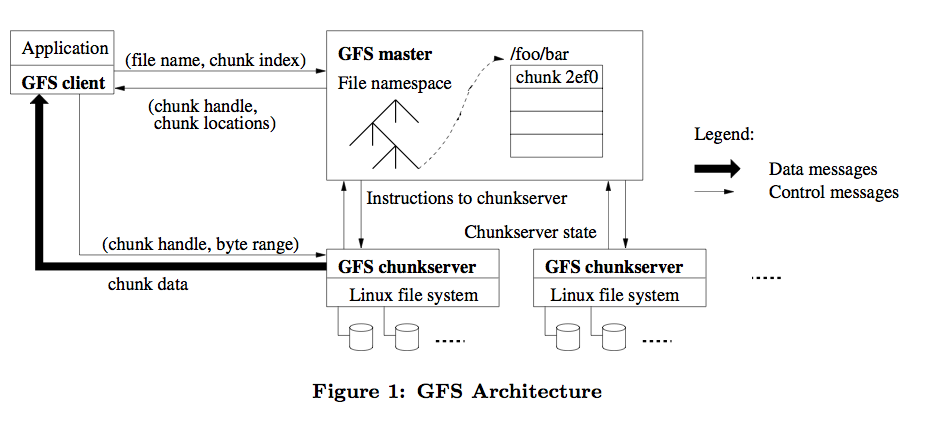
\includegraphics[scale=0.5]{images/gfs}
\caption{Architektura Google File System \cite{gfs}}
\label{fig:3v}
\end{figure}

\section{BigTable}
Jedná se o systém na uchovávání dat spoledčnosti Google, který je postavený nad Google File Systémem a jinými technologiemi společnosti Google. Jedná se o proprietární software, který není kdispozici mimo firmu Google, kromě možnost využívat tento sw jako část služby Google App Engine.  V roce 2006 opět google zveřejnil článek o BigTable \cite{bigtable}, avšak nyní s mnohem méně detaily, nežli u svého článku o GFS \cite{gfs}, kvůli obavám o přesné zkopírování jako u zmíněného systému. V době vydání článku bigtable obsluhoval více než 60 služeb firmy Google a škáloval několik Petabytů dat na několika tisici počítačích. BigTable umožňuje využívání MapReduce frameworku. Jedná se o první implementaci mnoho sloupcové, distribuované, multidimenzionální perzistentní seřazené mapy.  Google opět udal trend jakým se podobné systémy začali ubírat. Datový model BigTable v budoucnu inspiroval i tvůrce Apache Cassandra, která je hlavním tématem této práce a proto detaily ohledně datového modelu prozatím přeskočíme.

\section{MapReduce}
Je programovací model a framework prvně představený společností Google \cite{mapreduce} na zpracování velkého datasetu. Uživatel specifikuje mapovací funkci, která zpracuje páry (klíč, hodnota) a vygeneruje přechodné páry (klíč hodnota), které jsou pak předané redukovací funkci, která sloučí všechny mezi-hodnoty se stejným mezi-klíčem. Mnoho příkladů z reálného světa, lze převézt do tohoto paradigmatu. Výhodou těchto funkcionálně napsaných programů je, že jsou automaticky velice paralelizovatelné. Systém se stará o detaily distribuce dat a rozhození jednotlivých uloh na jednotlivé počítače a obsluhuje chyby a neočekávané stavy. toto umožňuje programátorům i s velice malou znalostí paralelního programování napsat vysoce paralelní a efektivní programy. 

Toto paradigma se stalo v nejdůležitějším stavebním kamenem pro zpracovavání BigData. Díky tomuto mechanizmu jsme schopni zpracovávat Terabyty dat rychle a efektivně a vypočítaný výsledek znovu uložit do databáze. Veškeré postupy zpracování BigData jsou přímo, či nepřímo založené na MapReduce. 

\begin{figure}[!h]
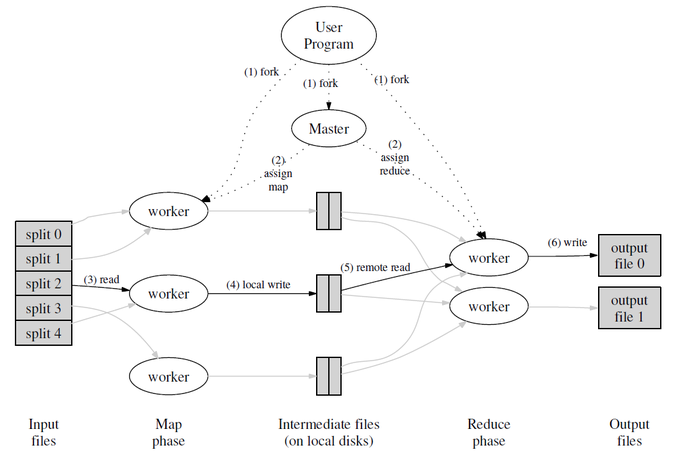
\includegraphics[scale=0.6]{images/mapreduce}
\caption{MapReduce schéma \cite{mapreduce}}
\label{fig:mapreduce}
\end{figure}

\newpage

\section{NoSQL}
Se zkratkou SQL se můžeme u relačních databázových systémů. Zkratka NoSQL neznamená pravý opak, písmena \uv{No} znamenají \uv{Not Only}, tedy ne pouze. Jedná se o databázový koncept, který se vyskytuje u nerelačních databází. V tomto konceptu datové úložiště i zpraování dat používají jiné prostředky, než běžné tabulkové schéma relační databáze. Výhody tohoto konceptu jsou jednoduchá desihn a horizontální i vertikální škálovatelnost. NoSQL databáze často podporují také podmnožinu jazyka SQL a většinou se jedná o jednoduché funkce jako vkládání a velice jednoduché výběry. Některé NoSQL databáze mají i velice odlišný ukládací model, například (stromový, grafový) tím padem je složitost  pro různé operace odlišná. Nejčastější podobu má NoSQL databáze formou klíč hodnota, čili mapa. Podle dosavadních informací lze říci, že Google BigTable je tedy NoSQL databáze. Mezi charakteristiky NoSQL databází můžeme zahrnout

\begin{itemize}
\item \textbf{Datový a dotazovací model} - jak již bylo řečeno NoSQL databáze se liší způsobem udržování dat a  dotazováním nad nimi
\item \textbf{Perzistence} - Ne všechny NoSQL datbáze ukládají svá data na disk, některé databáze běží pouze v operační paměti.
\item \textbf{Rozhraní} - Některé databáze komunikují skrze REST rozhraní a některé pomocí binárních protokolů 
\item \textbf{BASE} - Tak jako relační databáze využívají vlastnosti ACID (Atomic Consistent Isolation Durability) tak v NoSQL je ekvivalentem BASE (Basically Available, Soft state, Eventual consistency) kde každá NoSQL databáze garantuje jednotlivé vlastnosti různými mechanizmy a nastaveními nebo jsou již od základu navržené s danými vlastnostmi.   
\end{itemize}


NoSQL databáze jsou dalším základním stavebním kamenem BigData. NoSQL databáze jsou často kompatibilní s MapReduce konceptem, čímž tvoří ideální dvojici pro uchovávání a zpracování velkého množství dat. 



\chapter{BigData Platforma Apache}

V předchozí kapitole jsme se seznámili s technickými principy a postupy, které se uplatňujív BigData konceptu. V tét kapitole se budu zabývat jedním z hlavních témat práce a tou je open source řešení pro platformu BigData od organizace Apache Foundations, také známý jako Apache Big Data stack. Tento stack se skládá z několika aplikací, které až na jednu výjimku na sobě nejsou nikterak závislé. V záběru této kapitoly se budu důkladně věnovat pro nás nejdůležitější části tohoto stacku a tím je NoSQL databázový systém Cassandra.

\section{Hadoop}




Hadoop je softwarová knihovna napsaná v programovacím jazyce Java a umožňuje distribuované zpracování velkého množství dat napříč clusterem pomocí jednoduchých programovacíh modelů- Je navržený aby dobře škáloval cluster tvořící jeden až několik tisíc počítačů, kde každý nabízí lokální výpočetní výkon a úložiště dat. Hadoop řeší problémy s hardwarem na aplikační vrstvě a tudíž je možné navrhovat vysoce dostupné služby na clusterů počítačů, aniž bychom se museli strachovat výpadků. Jeho 4 komponenty tvoří nejpodstatnější část pro celou analytickou práci s  daty. A všechny ostatní aplikace přímo, čí nepřímo některé části Hadoopu používají nebo jsou na nich dokonce založeny. Jaké tedy jsou tyto 4 komponenty hadoopu ?


\begin{figure}[h]
\centering

\includegraphics[scale=0.15]{images/hadoop}
\caption{Logo Apache hadoop}
\label{fig:yarn}

\end{figure}


\subsection{Hadoop Commons}
Jedná se pouze o základní sadu nástrojů podporujícíc a propojující ostatní moduly Hadoopu.


\subsection{Hadoop File System (HDFS)}
Jedná se o open source distribuovaný filesystém, jehož některé prvky vychází z dříve zmíněného GFS. HDFS umožňuje uložit velké množství dat mezi jednotlivé uzly.  HDFS umožňuje velice dobré škálování s rostoucím objemem dat. Ostatní technologie z Apache Big Data Stacku filesystém využívají ke sběru a ukládání výsledků jejich analytických procesů. HDFS cluster se skládá primárně z NameNode, který řídí filesystemová metadata a z DataNodů, které data uchovávají. 

\subsection{Hadoop MapReduce}
MapReduce jsme zmínili výše a jen zopakuji, že se jedná o programovací paradigma a framework na paralelní zpracování dat. Nabízí API, díky kterému můžeme jednoduše programovat naše vlastní MapReduce operace. Tento framework nabízí základní kostru, kterou programátor doplní a o vše ostatní se stará samotná knihovna. Přesto všakveškerá logika programu zavisí na programátorovi. 

\subsection{Hadoop YARN}
Tento modul se stará o plánování jednotlivých MapReduce programů a o správu dostupných zdrojů v celém clusteru a rozhoduje jaká data se kam budou posílat a počítat. Základní Architektura YARNu má za myšlenku mít jeden globální uzel, který se nazývá \uv{Resource Manager} a Pro každý běh aplikace mít tzv. \uv{Application Master}, který má na starosti komunikaci s \uv{Node Managery} a dohlížením nad spouštěním jednotlivých Tasků. Resource Manager se skládá ze 2 hlavních komponent Plánovače a Aplikačního manažera. Plánovač je zodpovědný za alokování zdrojů pro různé běžící aplikace. Aplikační manažer je zodpovědný za příjem nových MapReduce programů a jejich správné zařazení. NodeManager je agent běžící na každém stroji, která je zodpovědný za aplikační kontejnery a monitoruje stav dostupných prostředků stroje a ohlašuje se Resource Manageru, který tak má potřebné informace k přerozdělování nových úkolů.

\begin{figure}[h]
\centering
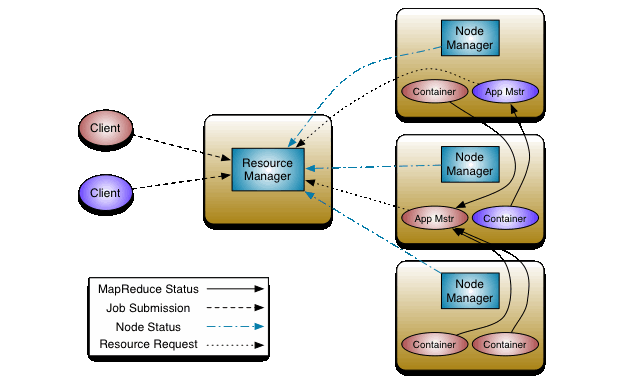
\includegraphics[scale=0.7]{images/yarn_architecture}
\caption{Architektura Hadoop YARN}
\label{fig:yarn}

\end{figure}



\newpage 

\section{HBase}
Je NoSQL databázový systém, který je založený na principu Google BigTable. Jedná se o druhou nejpoužívanšjí NoSQL databázi v Apache Big Data Stacku. Implementačně je zavíslá na HDFS, který používá k ukládání dat. Výhodou je velice jednoduhá a rychlá integrace s Hadoop MapReduce. HBase sdědil po Hadoopu i jeho Master-Slave architekturu.


\section{Hive}


Apache Hive je data warehouse infrastruktura postavená na vrchu Hadoopu na poskytování analýzy a dotazování se nad daty. Původně byl tento software vyvinut ve společnosti Facebook. A nyní se jeho starají společnost jako je NetFlix a Amazon. Hive podporuje anaýzu velkých datasetů uložených v HDFS nebo HDFS-kompatibilních systémech jako například (CassandraFS nebo Amazon S3). Syntaxe jeho dotazovacího jazyka HiveQL je velice podobná SQL a proto ho mohou inženýři ovládající tento jazyk velice brzy ovládnout.HiveQL nabízí programátorům prostředky, které nejsou běžně v NoSQL databázích dostupné jako například funkce JOIN. 

\begin{wrapfigure}{r}{0.5\textwidth}
  \centering
    
\includegraphics[scale=0.5]{images/hive_logo}
\caption{Logo Apache Hive}

\end{wrapfigure}

Hive funguje na principu, že si dotaz přeloží a převede do kodu kompatibilního s Hadoop Mapreduce a výsledný program následně spustí na Hadoop clusteru. Obrovskou výhodou je, že programátor dostává v podstatě s nulovým snažením hotový MapReduce program, který by jinak musel zdlouhavě psát, což umožnuje být vysoce efektivní. Hive si standardně ukládá metadata do embedované databáze Derby. Podporuje pokročilejší funkce jako například Indexy, kompresi nebo uživatelem definované funkce (UDF) samozřejmostí jsou standardní matematické a řetězcové funkce aplikovatelné v HiveQL dotazech. 



\section{Pig}


Pig funguje na stejném principu jako Hive. Tedy , že převede vámi napsaný kód do hotového MapReduce řešení a tento kód spustí nad Hadoop clusterem. Tato knihovna byla napsána ve firme Yahoo a později opensourcována pod Apache foundation. Pig používá svůj vlastní jazyk pojmenovaný Pig Latin a oproti HiveQL nemá s SQL moc společných rysů. Latin se spíše podobá funkcionálním jazykům. Pig a Hive dělají tedy stejné věci, tak proč používat obojí? Je to spíše volba osobních preferencí, či preferencí vašeho vývojářského týmu. S oběma technologiemi lze dosáhnout stejných výsledků. Přesto má Pig lepší uplatnění v případě tvorby komplikověnšjích data flow a HiveQL se více hodí pokud jsou potřeba Ad-Hoc dotazy. Přestože lze dosáhnout stejných výsledků s oběmi platformami, určitě doporučuji umět obě a použít Hive nebo Pig v konkrétních siuacích, kde mají lepší užití. 



\section{SolR}

Solr [Solar] je vyhledávací platformou odvozenou od Apache Lucene. Mezi její hlavní výhody patří:

\begin{itemize}
\item Pokročilý full-text vyhledávací engine
\item Optimalizace pro vysokoobjemový tok dat
\item Otevřené rozhraní pomocí XML,JSON nebo HTTP
\item Lineární škálovatelnost, automatická replikace indexu, auto failover a samoobnovení
\item Indexace v témeř reálném čase
\item Možnost doprogramování vlastních pluginů
\end{itemize}

Solr využívá Lucene index, což znamená, že je formát je striktně definovaný. Změna ve formátu indexu znamená reindexaci celého dokumentu. Díky lehkému nastavení a možnostem výstupu a pokročilými funkcemi jako je například GeoSpatial vyhledávání nebo facetové full text hledání, je SolR v komerční a open source sféře vyhledávacím enginem číslo 1.


\section{Squoop}

Tento nástroj je velice užitečný, protože ne vždy chceme mít všechna data pouze v NoSQL databázích a pokud to je možné, využití výhod relačních databází je logickou volbou. Apache Squoop je nástroj pro hromadnou migraci z HDFS (či kompatibilního) file systému do strukturovaných úložišt jako například: relačních databází. Přesun dat je navržený obousměrně stejně tak můžeme využít Squoop k migraci dat z  relačních databází do HDFS (a kompatibilních) systémů. Výhodou je vysoká efektivita a nízká časová investice oproti psaní vlastních migračních scriptů.

\section{Mahout}

Mahout je slovo, které pochazí z Hindi a jeho překladem do češtiný získáme spojení jezdec na slonovi. Slonem se v BigData komunitě myslí projekt Apache Hadoop, který má slona ve svém logu a je s tímto zvířetem neodmyslitelně spojený. Projekt Mahout se snaží svým metaforickým názvem naznačit využívání hadoopu k vytvoření knihovny pro podporu škálovatelného \uv{Machine learningu}. Mahout je sada funkcí a algoritmů využívaných v odvětví machine learningu, naprogramovaných pomocí Hadoop MapReduce paradigmatu. Primární zaměření Mahoutu je na odvětví kolaborativního filterování, clusterování a klasifikace dat. Mahout také obsahuje vysoké množství matematických funkcí a algoritmů z oblasti lineární  algebry a statistiky. V současné době lze využít Mahout na tyto základní způsoby užití. Doporučovací funkce na základě uživatelského chování, rozřazování dokumentů do clusterů na základě shody v obsahu a Klasifikace dokumentů na základě již uložených kategorizovaných dokumentů. 

\section {ZooKeeper}

Autoři projektů v rámci Apache foundations a především ti zaměření na projekty BigData stacku mají pro metafory a různá symbolická spojení velkou slabost. Jak názvy a loga projektů napovídají, velká část projektů má v názvu nebo logu nějaké zvíře, či referenci na něj. Zároveň uhlídat a spravovat byť malý ale distribuovaný systém, může být velký chaos a proto je potřeba ten správný hlídač. ZooKeeper v překladu tedy hlídač zoo je nástroj pro správu a konfiguraci distribuovaných systému z platformy Apache BigData. 




\chapter{Vhodné případy užití}
\section{Analýza Access logů}
\section{Image Servery}


\chapter{Implementace některých případu užití}
\section{Testovací prostředí}
\section{Implementace Access Log analyzéru}

\begin{conclusion}
	%sem napište závěr Vaší práce
\end{conclusion}

\nocite{*}
\bibliographystyle{csn690}
\bibliography{mybibliographyfile}

\appendix

\chapter{Seznam použitých zkratek}
% \printglossaries
\begin{description}
	\item[GUI] Graphical user interface
	\item[XML] Extensible markup language
\end{description}

\chapter{Obsah přiloženého CD}

%upravte podle skutecnosti

\begin{figure}
	\dirtree{%
		.1 readme.txt\DTcomment{stručný popis obsahu CD}.
		.1 exe\DTcomment{adresář se spustitelnou formou implementace}.
		.1 src.
		.2 impl\DTcomment{zdrojové kódy implementace}.
		.2 thesis\DTcomment{zdrojová forma práce ve formátu \LaTeX{}}.
		.1 text\DTcomment{text práce}.
		.2 thesis.pdf\DTcomment{text práce ve formátu PDF}.
		.2 thesis.ps\DTcomment{text práce ve formátu PS}.
	}
\end{figure}

\end{document}
